\documentclass[a4paper,10pt]{article}
\usepackage{a4wide,graphicx,enumerate}

\title{Report on Second Order Solvers for the 1D Wave Equation}
\author{Girish Nivarti (50951094)}
\date{\today}

\begin{document}
\maketitle

\emph{Problem:} Solve the one dimensional wave equation given by:
\begin{equation}
  \frac{\partial T(x,t)}{\partial t} +   u\frac{\partial T(x,t)}{\partial x} = 0 
\end{equation}

using the finite volume method with given initial condition, T(x, 0) = sin(2$\pi$x). Compare the computed solution to the analytically solved exact solution:
\begin{equation}
  T(x,y) = sin(2\pi(x - 2t))
\end{equation}


\emph{Solution:} 
\begin{enumerate}[I]
\item The error in numerical solutions using 20, and 40 cells has been plotted in Fig.~\ref{errors}. The solution profiles have been plotted in Fig.~\ref{solution}. The $L_2$ norms of the solutions are, 0.298335722822351 for 20 cells, and 0.0783745912112995 for solution using 40 cells. The $L_2$ norm reduces with increasing mesh size. It drops below $10^{-3}$ (value of norm 0.000990862339100897)for 357 control volumes, and below $10^{-4}$ (value of norm 0.0000999594805847065) for 1124 cells. The accuracy of the code is reasonable, however, there is a phase lead in the numerical solution which is a sizeable fraction (5\%) for low cell numbers. A log plot of error norms versus time step for 40 control volume mesh, as well as a log plot of error norm versus cell size for CFL 0.3 were plotted. The trend plotted in Fig.~\ref{norms} and exhibited a power law fit of second order. The solution norm shows a low order dependence on time step variation and has not been plotted.

%% 0.1 0.00125 0.0728551979366369
%% 0.2 0.0025 0.0739606127747022
%% 0.4 0.005 0.0783745912112995

\item A graph showing various stability profiles has been plotted. For purpose of clarity and to demonstrate what happens around that point, a value that is slightly beyond borderline is shown in Fig.~\ref{stability} to highlight the behaviour of numerical solution near stability boundary. A borderline value (of CFL) for stability was established by hit and trial. About 153 time steps ($\Delta t = 0.0065625$) were taken for the highest possible CFL number that produced a solution that had no recognizable changes from the exact solution. However, the $L_2$ norm changes abruptly at CFL = 0.5 - even a small increase beyond this number (which happens to be the analytically calculated maximum CFL) changes the norm by a sizable fraction. However, the plots show a 0.525 CFL number as being borderline based on observable properties of the graph. $L_2$ norms of these different solutions have been tabulated in Table~\ref{table:norm}. This is roughly consistent with an eigenvalue analysis.



\item The Superbee limiter was implemented to evaluate fluxes in the domain for both smooth solution (sine), and a discontinuous solution (square wave). A CFL number of $0.8 \times CFL_{max} = 0.42$ (where, $CFL_{max} = 0.525$ was used, as it was the observable maximum) was used for these calculations for a mesh with 100 control volumes. Plots of smooth solution (Fig.~\ref{smooth}), and discontinuous solution (Fig.~\ref{square}) have been made showing calculations using limited (Superbee) and non-limited flux evaluation.
\end{enumerate}

  \begin{table}
      \begin{center}
        \begin{tabular}{|l | l | l | r |}
          \hline
          CFL Number & Time Step ($\Delta t$) & $L_2$ Norm & Stability Character\\
          \hline
          0.3 & 0.00375 & 0.138003604480734 & Surely Stable \\
          0.525 & 0.0065625  & 0.177735260766837 & Borderline Stable \\
          0.528 & 0.0066 & 0.221828943126969 & Slightly Unstable \\
          0.54 & 0.00675 & 7521.55871620826 & Quite Unstable \\
          \hline
        \end{tabular}
        \caption{Stability characteristics of numerical solutions with different CFL numbers.}
        \label{table:norm}      
      \end{center}
    \end{table}

\begin{figure}
  \centering
  \includegraphics[width=0.6\textwidth, angle = -90]{../plots/temp/Temp.eps}
  \caption{Numerical solutions of the 1D wave equation using second order upwind spatial discretization, and two-stage Runge Kutta time marching scheme with different mesh sizes (20, and 40 control volumes) compared with the exact solution after 1 time unit. The $L_2$ norms of the solutions are, 0.298335722822351 for 20 cells, and 0.0783745912112995 for solution using 40 cells.}                
  \label{solution}
\end{figure}


  \begin{table}
      \begin{center}
        \begin{tabular}{|l | l | l | r |}
          \hline
          CFL Number & Exact Solution Character ($\Delta t$) & Flux Evaluation & $L_2$ Norm \\
          \hline
          0.42 & Smooth & Unlimited & 0.0369757641117924 \\
          0.42 & Smooth  & Superbee & 0.0276493801287461 \\
          0.42 & Discontinuous & Unlimited & 0.336394727433405 \\
          0.42 & Discontinuous & Superbee & 0.13283223625804 \\
          \hline
        \end{tabular}
        \caption{Solution error characteristics for smooth, and discontinuous solutions with, and without limiting. Interestingly the Superbee solution has lower norms in both smooth and discontinuous solutions. This is due to the phase lead that makes the unlimited solution have a bigger norm.}
        \label{table:norm2}      
      \end{center}
    \end{table}




\begin{figure}
  \centering
  \includegraphics[width=0.6\textwidth, angle = -90]{../plots/error/Error.eps}
  \caption{Errors in the numerical solution for 1D wave equation for meshes with 20, and 40 control volumes. Errors subside quickly with increasing control volumes yet oscillate about values making it difficult to find threshold mesh sizes for given $L_2$ norm order.}                
  \label{errors}
\end{figure}

\begin{figure}
  \centering
  \includegraphics[width=0.6\textwidth, angle = -90]{../plots/order/Order.eps}
  \caption{Errorn norms ($L_2$) of the numerical solution using second order upwind spatial discretization, and two-stage Runge Kutta time marching scheme has been plotted on a log scale for a range of mesh sizes. The $L_2$ norms fit the general trend with slope 1.99939233, while for some odd points, another trend with a slightly lower order (1.47052215) seems to exist.}                
  \label{norms}
\end{figure}

\begin{figure}
  \centering
  \includegraphics[width=0.6\textwidth, angle = -90]{../plots/stability/Stability.eps}
  \caption{Numerical solutions with different CFL numbers have been compared to highlight the behaviour of profiles with varying time step sizes. The solution is sensitive near the borderline making it difficult (not impossible) to pin-point borderline value. The profile for a near borderline yet unstable solution has been plotted to show the changes in solution near the borderline.}                
  \label{stability}
\end{figure}
 
\begin{figure}
  \centering
  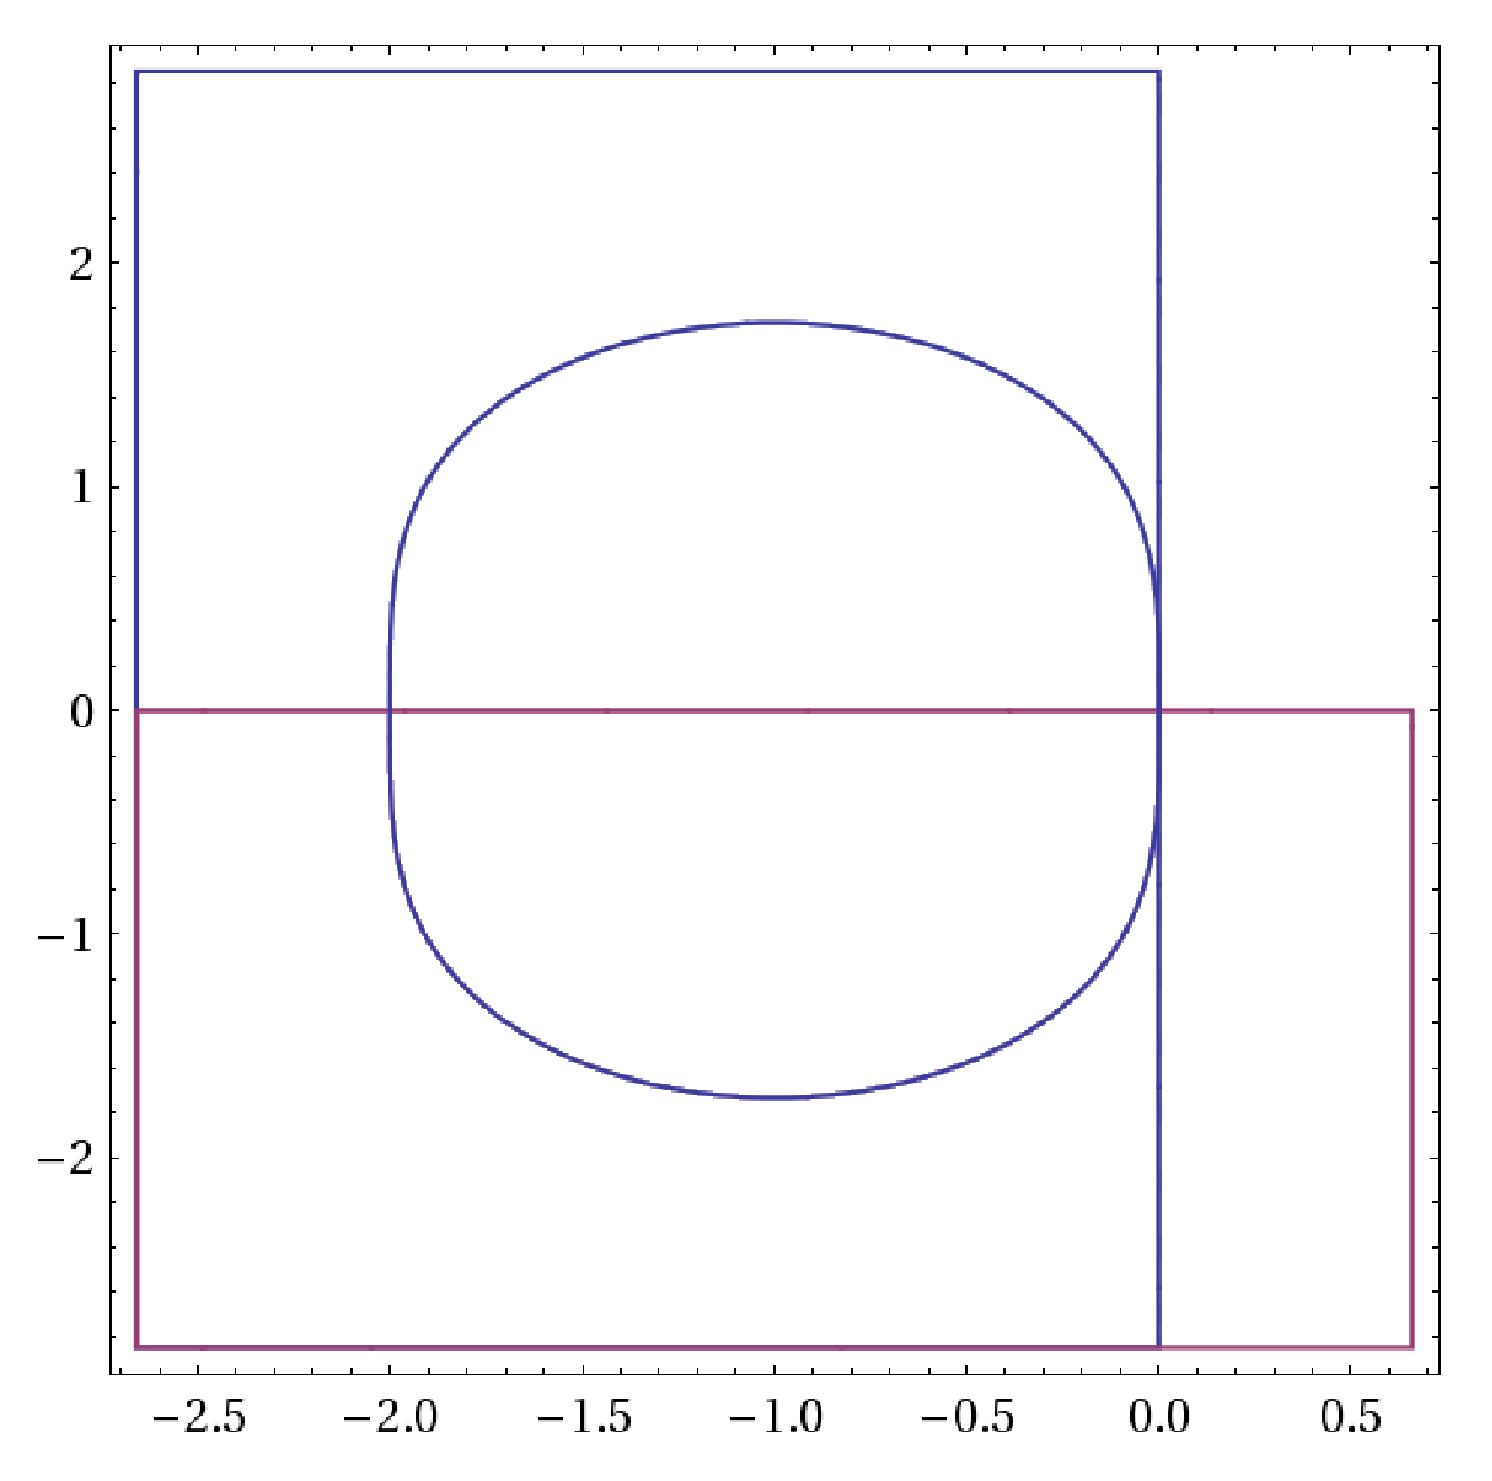
\includegraphics[width=0.6\textwidth]{../plots/eigenvalue/eigen1.eps}
  \caption{Two stage Runge-Kutta time marching scheme has the given contour for amplification factor, $\sigma = 1$ with the minimum real value being $\lambda \Delta t = -2$. The domain for second order upwind has a contour that is primarily dictated by the real values of CFL number. The minimum value is $-4\frac{u\Delta t}{\Delta x}$. Hence, that gives $CFL_{max}\leq 0.5$.}                
  \label{rk2}
\end{figure}
 
\begin{figure}
  \centering
  \includegraphics[width=0.6\textwidth, angle = -90]{../plots/smooth/Smooth.eps}
  \caption{Profiles of numerical solutions with (Superbee), and without flux limiting for a 100 control volume mesh size have been shown to demonstrate failure of flux limiting which is based on purely discontinuous solutions. ENO schemes prove useful for solution exhibiting mixed character.}                
  \label{smooth}

\end{figure}
 
\begin{figure}
  \centering
  \includegraphics[width=0.6\textwidth, angle = -90]{../plots/square/Square.eps}
  \caption{The Superbee flux limiting proves to be highly accurate in comparison to a non-limited scheme (for a 100 control volume mesh size) in solving a square wave.}                
  \label{square}
\end{figure}
 
 
    %% \begin{table}
    %%   \begin{center}
    %%     \begin{tabular}{|l | c | c | r|}
    %%       \hline
    %%       Mesh Size & Convergence Criteria & Iterations & $L_2$ Norm\\
    %%       \hline
    %%       10x10 & $10^{-8}$ & 120 & 0.00245705 \\
    %%       20x20 & $10^{-9}$ & 410 & 0.000638619\\
    %%       40x40 & $10^{-10}$ & 1629 & 0.000161223\\
    %%       80x80 & $10^{-11}$ & 6519 & 0.0000404044\\
    %%       \hline
    %%     \end{tabular}
    %%     \caption{Convergence beahviour of solutions using point Gauss-Seidel iterative scheme with over-relaxation (1.5)}
    %%     \label{table:norm}      
    %%   \end{center}
    %% \end{table}
    
    %% \item Poisson problem in pressure calculation for incompressible flows: The following equation was solved in a uniform grid  spanning the domain 1x1 in dimensions.
    %% \begin{equation}
    %%   \frac{\partial^2 P(x,y)}{\partial x^2} +   \frac{\partial^2 P(x,y)}{\partial y^2} = -{\left\{\frac{\partial u}{\partial x}\right\}}^2 +  2{\frac{\partial u}{\partial x}}{\frac{\partial v}{\partial y}} + {\left\{\frac{\partial v}{\partial y}\right\}}^2
    %% \end{equation}
    
    %% with the following velocity field and given boundary conditions.
    %% \begin{eqnarray}
    %%   u = x^3 - 3xy^2\\
    %%   v = -3x^2y + y^3
    %% \end{eqnarray}
    %% The source variation across the domain was simplified to the expression:
    
    %% \begin{equation}
    %%   S = -18{(x^2 + y^2)}^2
    %% \end{equation}
    %% \begin{table}
    %%   \begin{center}
    %%     \begin{tabular}{|l | c | r|}
    %%       \hline
    %%       Mesh Size & Convergence Criteria & Iterations\\
    %%       \hline
    %%       20x20 & $10^{-8}$ & 1002\\
    %%       40x40 & $10^{-8}$ & 2936\\
    %%       80x80 & $10^{-8}$ & 12238\\
    %%       \hline
    %%     \end{tabular}
    %%     \caption{Convergence behaviour of finite volume solutions of Poisson problem in pressure solved using point Gauss-Seidel scheme with over-relaxation 1.5}
    %%     \label{table:norm2}      
    %%   \end{center}
    %% \end{table}

    
    %% The ASME procedure for analysis of error and estimation of order was implemented for values of P($\frac{1}{2},\frac{1}{2}$) using 3 different meshes (20x20, 40x40 and 80x80) with constant grid refinement factor, r = 2 to simplify error estimation. With a maximum change per iteration of Gauss-Seidel taken as $10^{-7}$, the apparent order of the scheme was calculated as $\mathcal{O} \sim 1.75002$ and the solution was extrapolated to: $4.93743 \pm 2.35637 \times 10^{-5}$ taking iterations of 859, 2936, and 10173 respectively. The same scheme was run for a lower ($10^{-8}$) tolerance for the maximum solution change per solution, where the values obtained for P($\frac{1}{2},\frac{1}{2}$) stopped fluctuating. The apparent order for this scheme was improved to $\mathcal{O} \sim 1.972644$ and the extrapolated solution was $P = 4.9374927 \pm 1.633160 \times 10^{-5}$ i.e. a smaller error bound.
\newpage
\emph{Comments:}
\begin{itemize}
\item A phase lead is seen in the RK2 solution of the smooth function (unnoticeable in the discontinuous case due to other predominant errors). In the solution with 20 control volumes, a single time step (5\%) lead was noticed, and with 40 control volumes the solution leads by 3 time steps (3\%). 

\item  While implementing the Superbee flux limiting, as an experiment, the corner points in the $\Psi$ - r curve, were assigned to different parts of the curve. For example the point (r = 0.5, $\Psi$ = 1) can be assigned to curves $\Psi$ = 2r, or $\Psi$ = 1. To my disappointment, there is no significant change by changing where this corner point lies.

\item The odd trend of norms can be attributed to the irregular values of dt obtained for certain mesh sizes that make the errors in floating point propagate and finally cause the time marching to carry to a time greater than required (inspite of running the loop based on number of time steps rather than on total time, and implementing a dt/2.0 correction factor mechanism). These errors are not $1^{st}$ order due to this correction factor, but are $\approx$ 1.5 order. It is difficult to eliminate such error.
  
\item For the last few control volumes, the value of r for limiting schemes depends on cells outside the domain. To handle this, ghost cells were created that contained values of the first few control volumes. In effect, the values along the wave are tabulated beyond the mesh. This  maintains periodicity and also allows us to use limiting for the last 2 cells. To add a caption of glory to our success, the $L_2$ norm decreases as well!

\item The $L_2$ norms provide an interesting picture of numerical solution as tabulated in Table~\ref{table:norm2}. Although the non-limited flux evaluation is considerably accurate with smooth solutions, the Superbee clearly fails by losing slope near extrema (Fig.~\ref{smooth}). But the $L_2$ norm in the discontinuous Superbee solution is greater than that for the smooth Superbee solution (looks - Fig.~\ref{square} - can be deceiving)! Indeed, the limited solution fails near the step change (in the square wave solution) by a greater amount than its failure near extrema in smooth solutions.

\item A crucial change was made on your suggestion, to force the time loop to stop nearest to the final time, T (\emph(tFinal) in code). This was done by counting number of integer time steps rather than calculating floating-point time. This makes a huge difference, because with comparing floating point numbers although there is a considerable drop in error on doubling the number of control volumes, but, it is noticed that the error norm fluctuates as the cells are increased further. It is difficult to pin-point a number for control volumes, for which error decreases steadily with increasing cells. In fact, there seem to be two modes of errors that steadily decrease with increasing control volumes but have different orders ($1^{st}$ and $2^{nd}$) of magnitude. 

\end{itemize}

\end{document}
